% Chapter Template

\chapter{Implementation and Results} % Main chapter title

\label{Chapter2} % Change X to a consecutive number; for referencing this chapter elsewhere, use \ref{ChapterX}

%----------------------------------------------------------------------------------------
%	SECTION 1
%----------------------------------------------------------------------------------------

\section{Implementation}
The code base worked with, was a direct Fortran90 implementation of the fingerprint algorithm proposed by \cite{Zhu2016}. The compiler used for all computation was the GNU Fortran compiler \cite{gnufortran}.

\subsection{Data}
The structures used for evaluating our methods were carbon-nitrate crystals. The data contained the positions of the atoms in cartesian coordinates and the lattice vectors of the unit cell. We thank Prof. Alireza Ghasemi for providing us with the data base of carbon-nitate structures that we have analysed.


\begin{figure}[p]
\center
\label{fig:structures}
\subfloat[8 atom unit cell]{%
  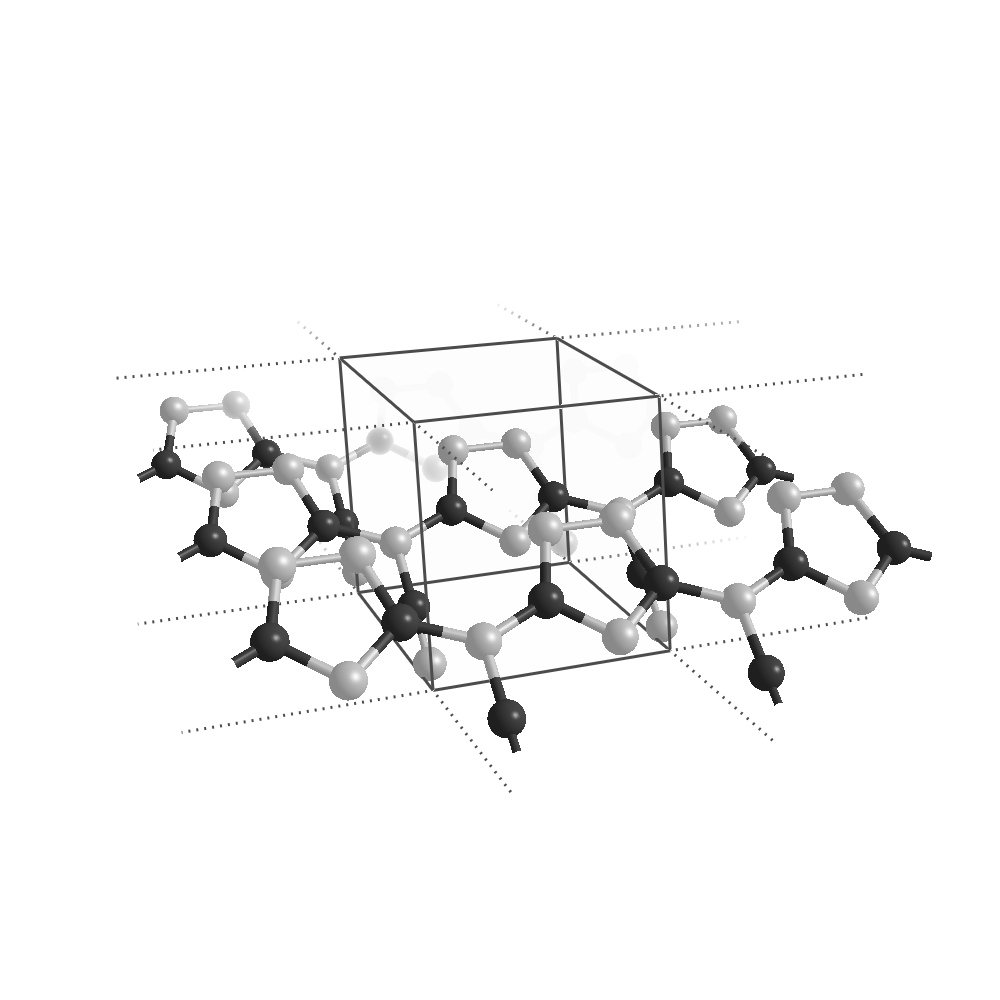
\includegraphics[clip,scale=0.3]{Figures/8structure.png}%
}

\subfloat[16 atom unit cell]{%
  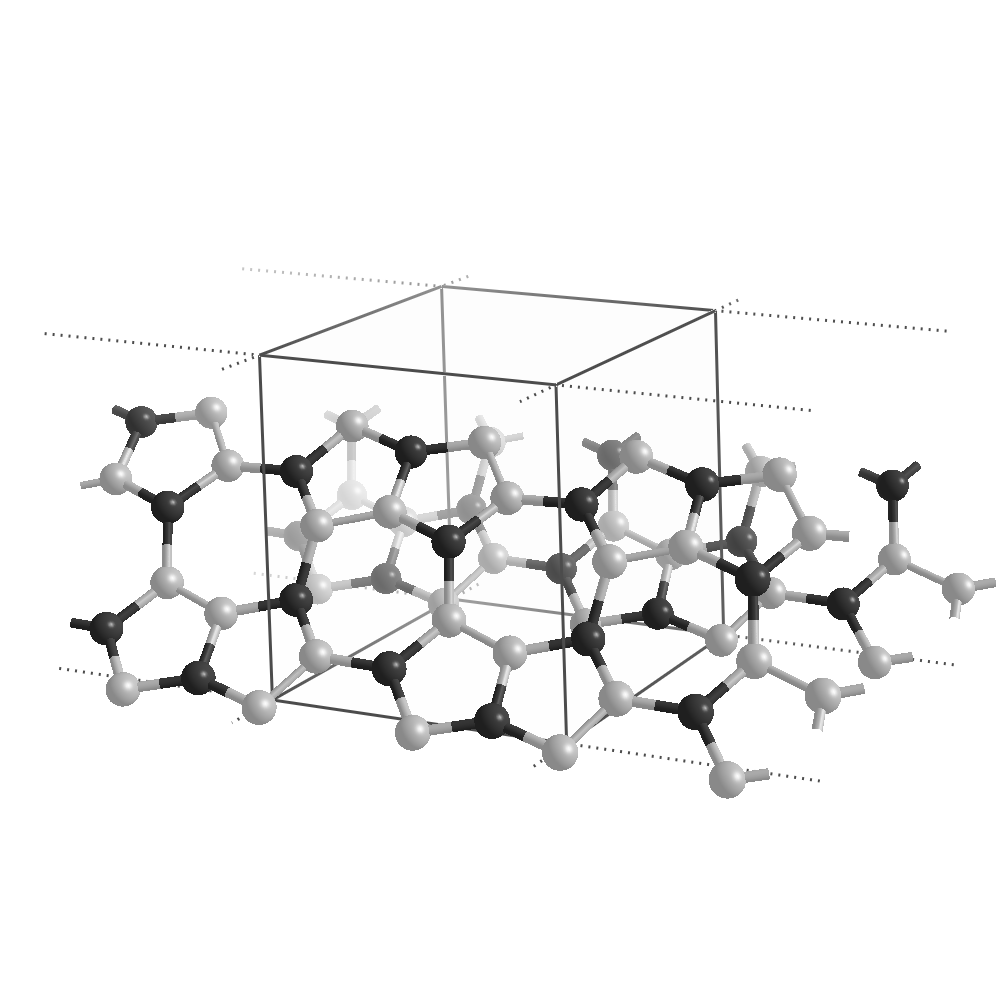
\includegraphics[clip,scale=0.3]{Figures/16structure.png}%
}

\caption{Example of the crystal structures used. C atoms are in black and N atoms in white. (A): Crystal sctructure with 8 atoms per cell. (B): Crystal structure with 16 atoms per cell.}

\end{figure}
\newpage
\subsection{Orbital Energies}
For calculating the overlap matrix (eq. \ref{ovrlap} ff.) the gaussian width $\alpha_i$ was originaly only dependent on the covalent radius of the respective atom type. This was further modified to respect the orbital eigenenergy of the respective orbital (eq. \ref{eq:const}). The values used were gathered from the NIST Atomic Reference Data for Electronic Stucture Calculations.

\begin{table}[h!]
\center
\label{table:energies}
\begin{tabular}{c|c|c}
            & \textbf{C} & \textbf{N} \\ \hline
2s {[}eV{]} & -0.500866  & -0.676151  \\ \hline
2p {[}eV{]} & -0.199186  & -0.266297 
\end{tabular}
\caption{2s and 2p orbital eigenenergies of N and C.}
\end{table}

The constant $C$ in (eq. \ref{eq:const}) was experimentally determined. To obtain a good resolution in comparing the fingerprints, the entries of the fingerprints should be reasonably large, but not to close to each other. One can see the effect of the constant $C$ out of (eq. \ref{eq:const}) by plotting the constant vs. the entries of the fingerprint.
With plots as seen in Figure \ref{fig:const} one can determine approximate boundaries for the constant. The entries should be reasonably distinct but still large enough to get a good resolution. The fine tuning was then done via maximizing the prediction accuracy. The final value used for all calculation was then $C=0.19$.


\begin{figure}[h]

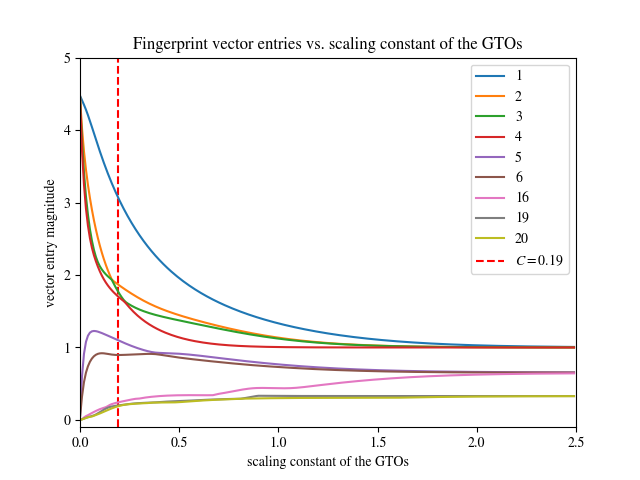
\includegraphics[width=\linewidth]{Figures/fpentry.png}
\caption{Plot of the fingerprint vector entries enumerated vs. the scaling constant of the GTO width.}
\label{fig:const} 
\end{figure}

\newpage
\section{Results}
\subsection{Landmark structures}

To calculate the landmark structures out of the fingerprints, we used a direct implementation of the maximum volume simplex method \cite{Behnam2020}. The task of this method should be to evaluate all atomar fingerprints given to it, and return the most distinct environments. These most distinct environments should furthermore each describe a different case of possible atomic environment regarding number of nearest neighbours (ligancy or coordination number) and type of nearest neighbours and their permutations. The method was evaluated on the set of 99 crystals with 8 atoms per crystal. Out of these 792 possible environments, the algorithm constructed a maximum volume simplex with 101 corners. A few of these landmark environments can be seen in Figure \ref{fig:landmarks1}, Figure \ref{fig:landmarks2}, Figure \ref{fig:landmarks3} and Figure \ref{fig:landmarks4}. The center atom is always either colored red for carbon and yellow for nitrogen in these depictions. Some of the atomic bonds were omited selectivly for visual clarity.


\begin{figure}[h!]

\center
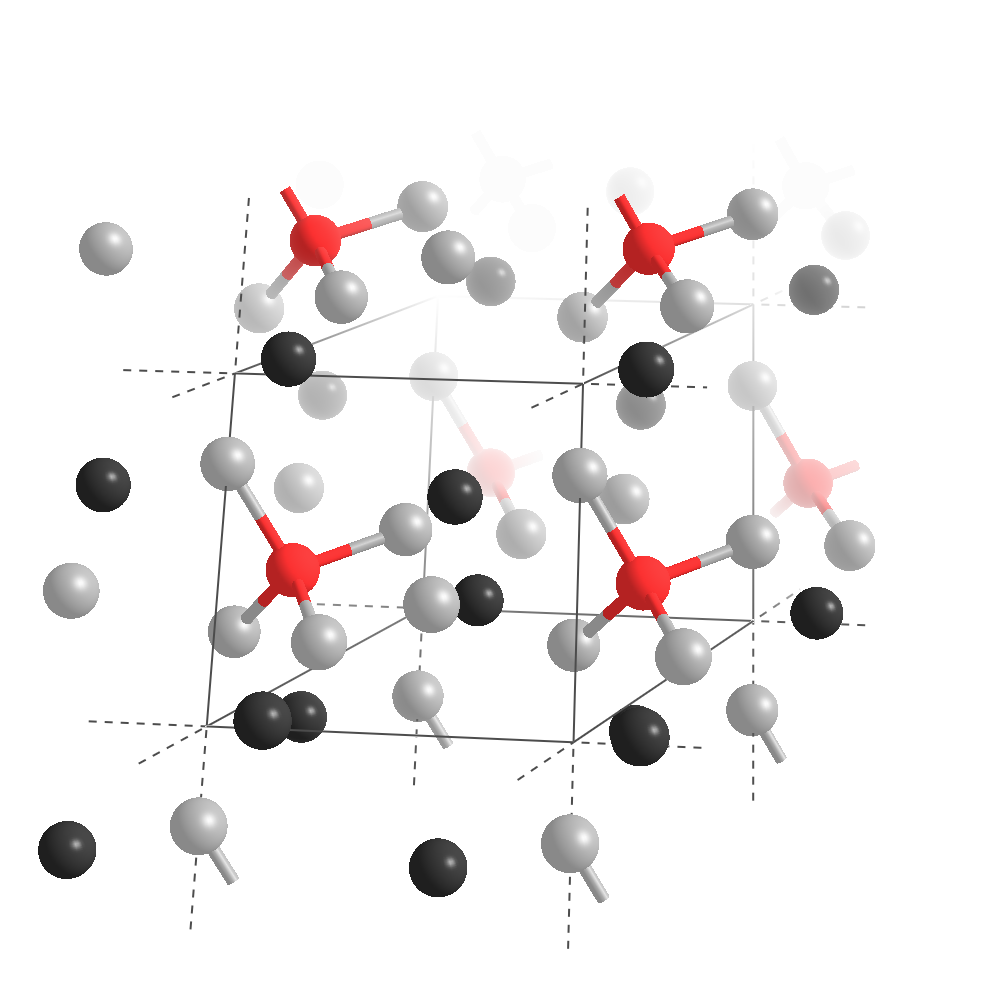
\includegraphics[width=\linewidth]{Figures/landmark1.png}
\caption{Landmark structure: Four times coordinated carbon with 4 nitrogen neighbours; black: carbon; white: nitrogen; red: carbon center atom. }
\label{fig:landmarks1}
\end{figure}

\begin{figure}[p]
\center
\subfloat[Once cooredinated nitrogen]{%
  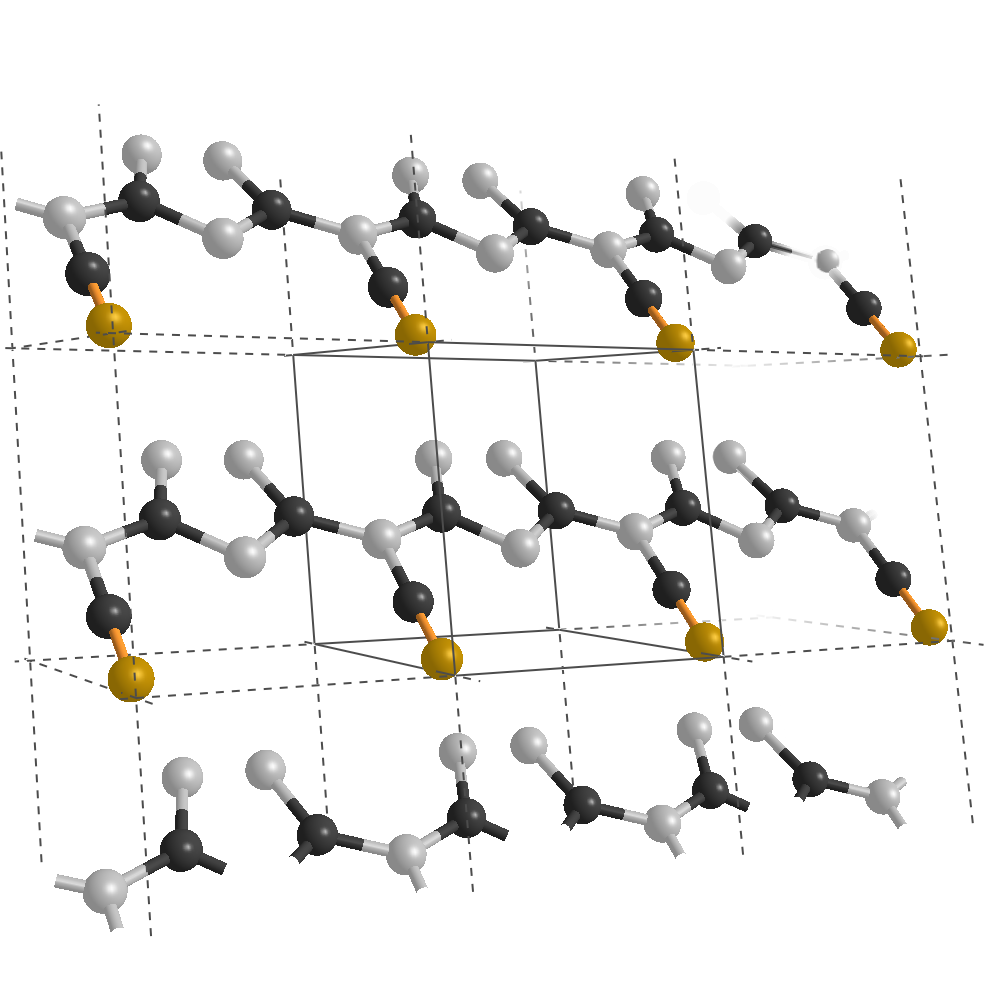
\includegraphics[clip,scale=0.3]{Figures/landmark2.png}%
}

\subfloat[Twice coordinated carbon]{%
  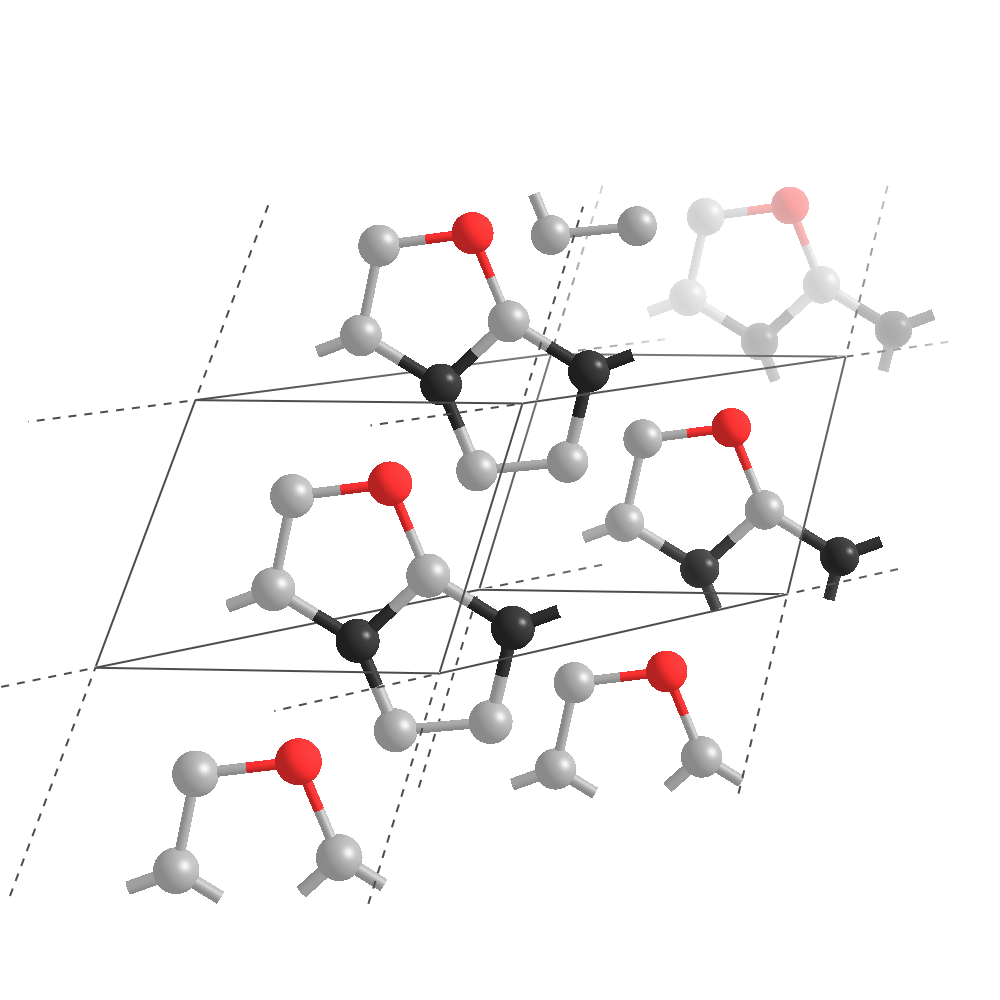
\includegraphics[clip,scale=0.3]{Figures/landmark3.png}%
}

\caption{Landmark structures: black: carbon; white: nitrogen; red: carbon center atom, yellow: nitrogen center atom}
\label{fig:landmarks2}

\end{figure}

\begin{figure}[p]
\center
\subfloat[three times cooredinated nitrogen with 3 carbon and 1 nitrogen neighbour]{%
  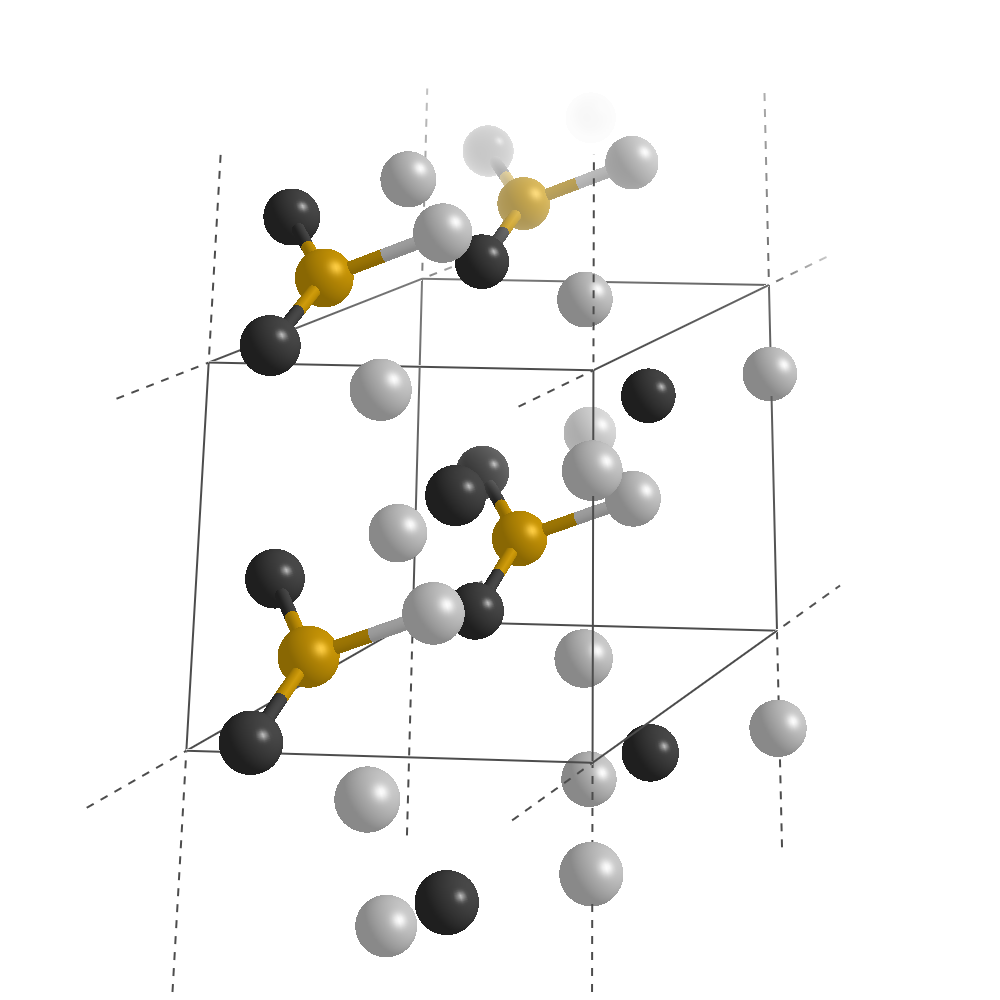
\includegraphics[clip,scale=0.3]{Figures/landmark4.png}%
}

\subfloat[three times cooredinated nitrogen with 3 carbon neighbours]{%
  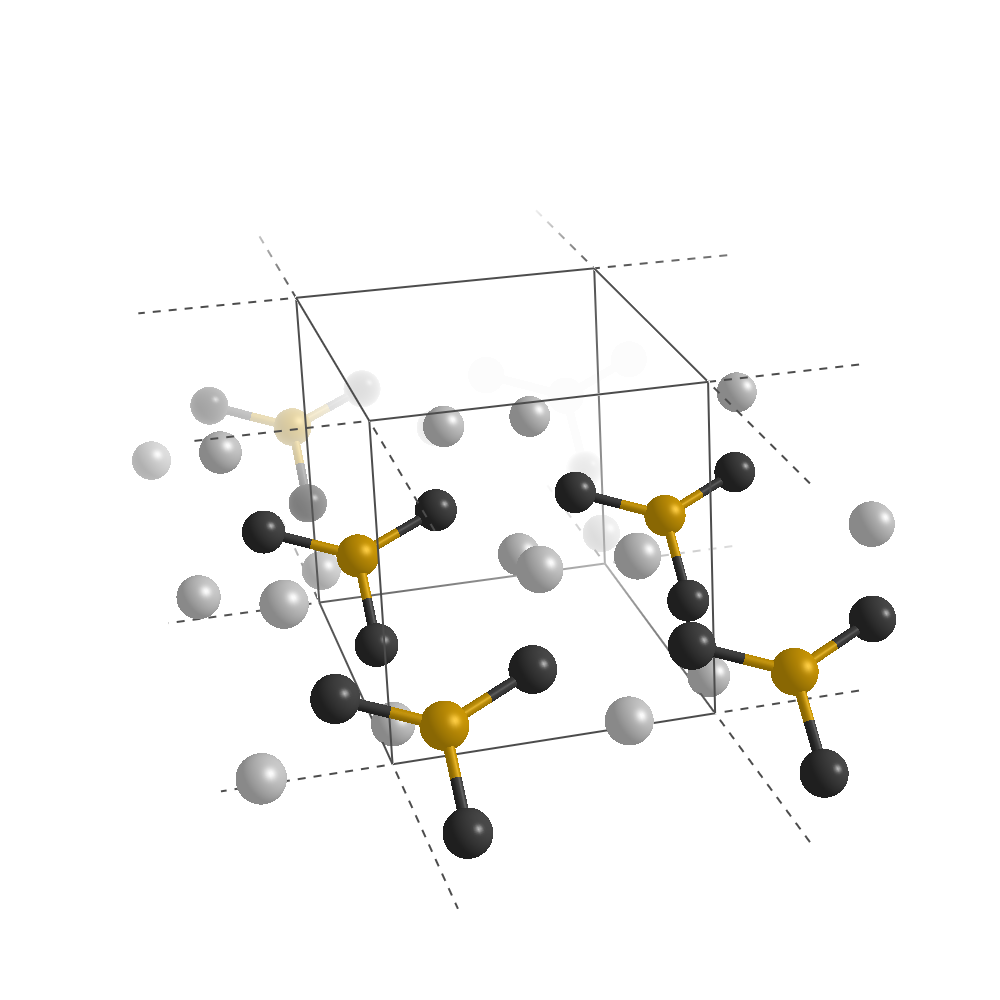
\includegraphics[clip,scale=0.3]{Figures/landmark5.png}%
}

\caption{Landmark structures: black: carbon; white: nitrogen; red: carbon center atom, yellow: nitrogen center atom}
\label{fig:landmarks3}

\end{figure}

\begin{figure}[p]
\center
\subfloat[twice coordinated carbon with 2 nitrogen neighbours]{%
  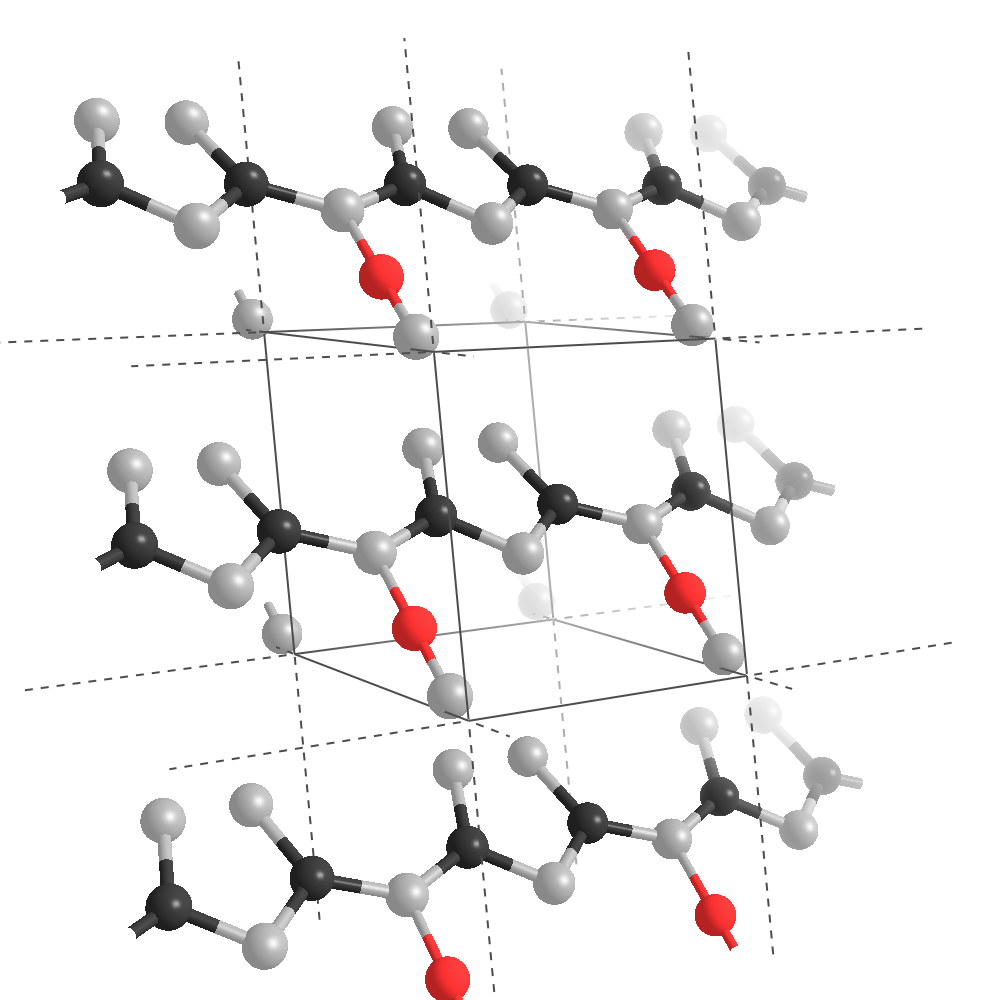
\includegraphics[clip,scale=0.3]{Figures/landmark6.png}%
}

\subfloat[three times cooredinated carbon with 3 nitrogen neighbours]{%
  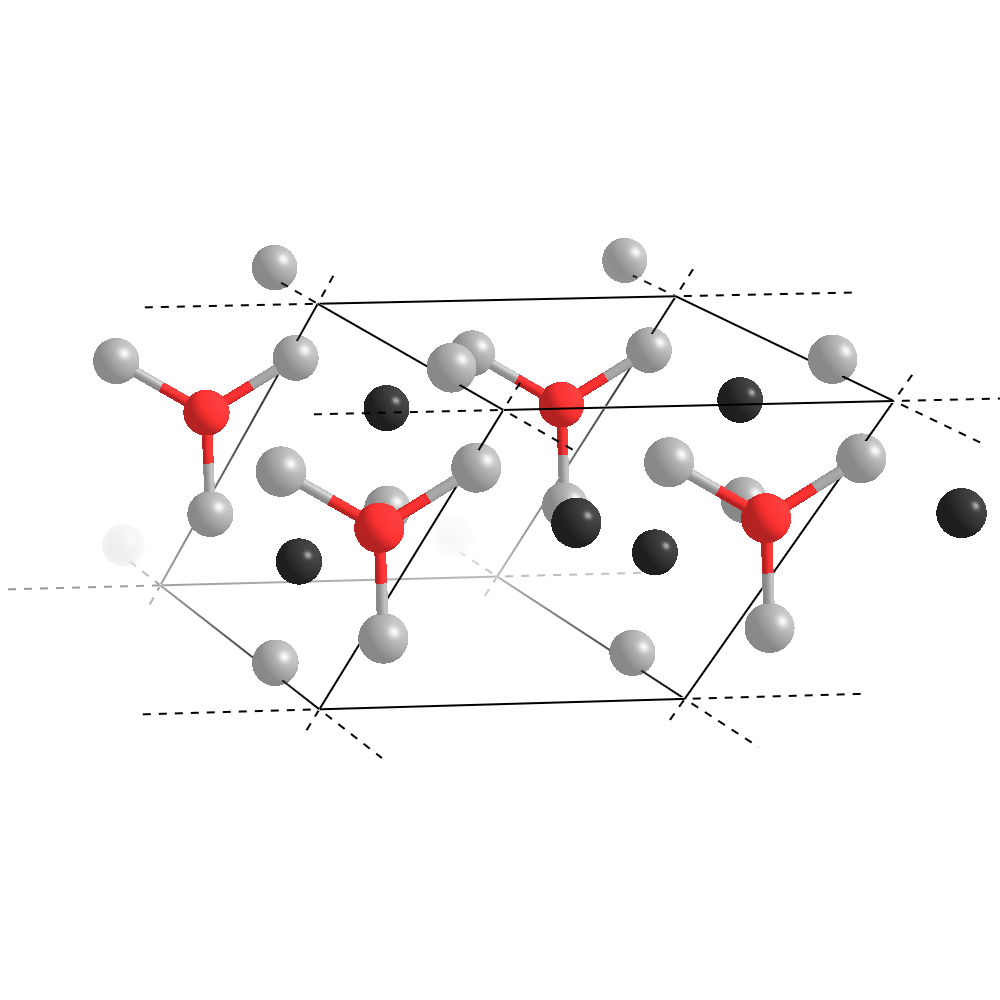
\includegraphics[clip,scale=0.3]{Figures/landmark7.png}%
}

\caption{Landmark structures: black: carbon; white: nitrogen; red: carbon center atom, yellow: nitrogen center atom}
\label{fig:landmarks4}

\end{figure}


\newpage
\subsection{Classification}
The classification was done in a relativly simple way. First, the \emph{trainings fingerprints} are calculated with the procedures mentioned earlier in this text. Then, the maximum simplex method is used to identify 101 landmark fingerprints. Of these landmark fingerprints, the type of center atom is stored aswell. Now, any atomar fingerprint can be compared to the landmark fingerprint via the euclidian distance. If the closest corner to our atom is a carbon, it predicts carbon. If the closest corner is a nitrogen, it predicts nitrogen.\\
\subsubsection{Training on eight atom crystals}
We trained our model first on a set of 99 configurations with 8 atoms per cell (3 Carbon and 5 Nitrogen). This was then validated on a set of 4949 crystals with 16 atoms per cell (6 carbon and 10 nitrogen) which gives us about 79'000 different environments to classify. The results of this procedure can be seen in Table \ref{table:res1}. 

\begin{table}[h!]
\center
\begin{tabular}{c|c|c|c}
classification & correct & false & correct (relative) \\ \hline
C              & 26497   & 4064  & 0.867              \\ \hline
N              & 45426   & 3197  & 0.934              \\ \hline
Total          & 71923   & 7261  & 0.908             
\end{tabular}
\caption{Classification results for the 4949 carbon nitrate crystals with 16 atoms per cell (79184 atoms in total) trained on 99 crystals with 8 atoms per cell.}
\label{table:res1}
\end{table}

One can see in Table \ref{table:res1} that the classification accuracy for carbon is considerably lower than that for nitrogen. The reason for this effect lies probably within the fact, that our trainings data contains about 1.6 times more nitrogen samples than carbon samples. So our model "knows" the nitrogen case better.

\subsubsection{Training on 16 atom crystals}
Next, we trained our model on a random selction of 63 16 atom crystals out of the 4949 crystals at our disposal. Then we classified the whole set of 16 atom crystals. The results can be seen in Table \ref{table:res2}.

\begin{table}[h!]
\center
\begin{tabular}{c|c|c|c}
classification & correct & false & correct (relative) \\ \hline
C              & 21151   & 3917  & 0.844              \\ \hline
N              & 45573   & 8543  & 0.842              \\ \hline
Total          & 66724   & 12460  & 0.843             
\end{tabular}
\caption{Classification results for the 4949 carbon nitrate crystals with 16 atoms per cell (79184 atoms in total) trained on 63 crystals with 16 atoms per cell.}
\label{table:res2}
\end{table}

Surprisingly, the accuracy is worse than before. Apparently training on a different (smaller) number of atoms per cell yielded better results than on training on the same. This of course can't be taken at face value since evaluating and comparing performance of machine learning methods is a very involved process which we will not get into in this report.



\subsection{Comparing to Supervised Learning with Random Forests}
Random Forests are intresting models for classification, since they require little configuration for reasonable predictions. The algorithm was first proposed by \citeauthor{Ho1995} \cite{Ho1995} and then extenden by \citeauthor{Breiman2001} \cite{Breiman2001}. It is a typical example of supervised learning, mapping input to output based on example input-ouput pairs. In our case, the example pairs are the either carbon or nitrogen labeled fingerprints in the trainings set.
The alrogrithm is very fast to train and very fast to validate. Training on a set of 52000 vectors willth 500 estimators on a consumer computer takes about 2 minutes. Once trained, the method can classify the 25000 fingerprints in a matter of seconds. We used the implementation of the Random Forest Classifier implemented for Python in scikit-learn by \citeauthor{scikit} \cite{scikit}. 

\begin{table}[h!]
\center
\begin{tabular}{c|c|c|c}
classification & correct & false & correct (relative) \\ \hline
C              & 8383   & 1475  & 0.850              \\ \hline
N              & 16128   & 407  & 0.975              \\ \hline
Total          & 24511   & 1881  & 0.929             
\end{tabular}
\caption{Classification results for the 26395 environments of the 16 atom structures averaged over 10 tries.}
\label{table:res3}
\end{table}

The results in Table \ref{table:res3} show an even greater divide between nitrogen and carbon which is again not surprising due to the imbalance of carbon to nitrogen in the training data. The Random Forest classifies the fingerprint vectors very well with an accuracy of about 93\% out of the box. This shows that the information we are looking for is clearly available in the fingerprint vector. The problem of Random Forests and supervised learning in general for our purposes is that it acts more or less as a black box. We can not deduce or induce physical meaning into or out of the work done by the Random Forest easily. It is however a powerful tool to see if the data contains the information we are looking for.

\section{Conclusion}
Being able to deduct the type of elements present in crystals just by looking at the atomic positions is something very useful in solid state physics. We demonstrated that the fingerprinting method and the maximum simplex method can be used to determine such quantities. The limitations with this method so far are that we are only looking at two different species of atoms and are therefore quite limited in what we can do. This could naturaly be extended to more atomic species, since the only parameters used were physical constants like the orbital eigenenergies and the covalent radii which are quantities very well known for most of the periodic table. There is also already a huge amount of data available to test and improve the method to suit tasks like classifying structures with more than two different kinds of atoms. Integrating both analytical methods such as the maximum simplex method and stochastic methods such as random forests and supervised learning in general shows huge potential in solid state physics.

% Training set size: 52789
% Validation set size: 26395
% (79184,)
% (79184, 400)
% [Parallel(n_jobs=1)]: Using backend SequentialBackend with 1 concurrent workers.
% [Parallel(n_jobs=1)]: Done 500 out of 500 | elapsed:  3.1min finished
% [Parallel(n_jobs=1)]: Using backend SequentialBackend with 1 concurrent workers.
% [Parallel(n_jobs=1)]: Done 500 out of 500 | elapsed:    3.2s finished
% The ratio of correct guesses is: 0.9227475941501857
% [[ 8316  1610]
%  [  429 16039]]